\documentclass[anon]{nesy2026}
% NeSy 2026 (PMLR/jmlr). Double-blind: [anon]. amsmath, amssymb, natbib, graphicx, url, algorithm2e auto-loaded.
\usepackage{booktabs}
\newcommand{\WMC}{\ensuremath{\mathrm{WMC}}}
\newcommand{\tw}{\ensuremath{\mathrm{tw}}}
\newcommand{\R}{\mathbb{R}}
\newcommand{\bC}[1]{\boldsymbol{#1}}

\title[Modular WMC for NeSy]{Modular weighted model counting for neuro-symbolic inference over large ontologies}

\clearauthor{\Name{Anonymous Author(s)} \Email{anon@example.org}\\
 \addr Anonymous Institution}

\begin{document}
\maketitle

\begin{abstract}
\noindent Neuro-symbolic learning couples a neural perception model with symbolic reasoning under a
\emph{conditional-independence assumption}: the perception model emits independent per-concept
marginals $p_i$, and the symbolic layer treats them as an independent product. This assumption is
known to impede optimization, distort uncertainty, and admit reasoning shortcuts. Repairing it
exactly means conditioning the factorized distribution on the symbolic theory, whose target
marginals $\mu_i$ are ratios of weighted model counts ($\WMC$); exact $\WMC$ is $\#$P-hard and, on a
description-logic ontology with tens of thousands of axioms, far beyond exact reasoning. We give the
soft, message-passing closure used in practice the two properties a deployable inference layer needs:
a correctness characterization and tractability at ontology scale. First, we show the
soft closure of the \emph{true-path theory} is loopy belief propagation -- hence the \emph{exact}
$\WMC$ marginal on the tree fragment for \emph{all} priors $q_i$, with error confined to
reconvergences (on a diamond the soft-OR update gives $9/10$ versus exact $5/6$, and the deployed
bidirectional closure deviates likewise); the proof is formalised in Lean~4. Second, the Gene Ontology
constraint graph has treewidth $12$/$37$/$269$ across its three namespaces, so monolithic exact
$\WMC$ is infeasible on the largest; yet cutting a ${\le}5\%$ reconvergence core makes $95$--$100\%$ of
the ontology exactly computable by a modular construction (each module exact to machine precision),
the bounded soft approximation confined to
the small core -- whose low-rank boundary joint a rank-$r$ separator message in turn dials to exact
(exact rank $6$ on a real GO core, versus $1024$ dense). Third, across the neuro-symbolic spectrum -- DeepProbLog (exact compilation is $\Theta(2^{\tw})$:
monolithic exact WMC compiles cc but not mf/bp), Scallop (top-$k$ drift concentrated exactly at
the reconvergences our theory identifies), and A-NeSI/NeSyDM (learned approximators that escape the
sampling collapse only by per-ontology training -- A-NeSI also needing samples of the exact $\WMC$
we compute -- so inapplicable to GO) -- ours is alone in being
both scalable and accuracy-characterized. We work in the EL fragment biomedical ontologies inhabit -- where exactness is
provable -- and show the same modular interface is the route to the disjunctive (SROIQ) regime where
the independence assumption bites hardest. A companion paper applies the layer to protein
function prediction.
\end{abstract}

\section{Introduction}
Neuro-symbolic (NeSy) learning combines the perceptual strength of neural networks with
the structure and verifiability of symbolic reasoning: a perception model maps inputs to
the truth values of symbolic concepts, and a symbolic layer reasons over them under a fixed
theory. Almost universally this coupling rests on a \emph{conditional-independence
assumption} -- the perception model emits independent per-concept marginals $p_i\in[0,1]$
and the symbolic layer treats the joint as the product
$q(\bC y)=\prod_i p_i^{y_i}(1-p_i)^{1-y_i}$
\citep{manhaeve2018deepproblog,xu2018semanticloss,ahmed2022spl} -- which makes the layer
differentiable and underwrites the semantic-loss and probabilistic-layer constructions much
of the field is built on \citep{xu2018semanticloss,ahmed2022spl,deraedt2020survey}.

The same assumption is now understood as a principal source of failure. Because the model
factorizes over concepts the theory couples, the product places mass on impossible
configurations and withholds it from theory-induced correlations. This \emph{impedes
optimization} (flattening or fragmenting the loss landscape), \emph{distorts uncertainty}
(the factorized posterior cannot represent a satisfied constraint's dependencies), and
admits \emph{reasoning shortcuts} (low loss through assignments that satisfy the theory but
not its semantics) \citep{vankrieken2024independence,marconato2023reasoningshortcuts,marconato2024bears}.
These pathologies are structural to the assumption and sharpen as the theory couples more
variables.

Repairing it has a clean meaning: condition $q$ on the symbolic theory $T$, yielding
$p_T(\bC y)\propto[\bC y\models T]\,q(\bC y)$, and read off the marginals
$\mu_i=p_T(y_i{=}1)=\WMC(T\wedge y_i;\bC p)/\WMC(T;\bC p)$, ratios of \emph{weighted model
counts} (WMC) -- exactly the semantic-probabilistic-layer object
\citep{ahmed2022spl,xu2018semanticloss}. But exact WMC is $\#$P-hard \citep{chavira2008wmc},
its compilation cost $\Theta(m\,2^{\tw})$ in the constraint-graph treewidth $\tw$
\citep{darwiche2002kcmap,darwiche2011sdd,bodlaender1993treewidth}; on a real ontology with
tens of thousands of axioms this is out of reach. Here deployed NeSy systems retreat to
soft, message-passing relaxations -- monotone closures, top-$k$ provenance -- whose
correctness is essentially never characterized. The field therefore faces a dichotomy: exact but
not scalable, or scalable but with no account of when, where, or how much they err.

This paper closes that gap for the \emph{true-path theory} -- the propositional grounding of
an ontology's hierarchical (is-a/part-of) and definitional axioms, the theory governing
protein function prediction over the Gene Ontology (GO)
\citep{ashburner2000go,geneontology2023}. It is the EL\textsuperscript{++} normal form of
subsumption and conjunction-definition axioms \citep{baader2005elenvelope,kazakov2014elk} -- the
OWL~2~EL profile the biomedical ontologies inhabit, and exactly the Horn fragment where this
exactness is provable (disjunction is the harder, SROIQ regime we return to in \S\ref{sec:nesy}) -- 
and the soft closure deployed against it is the monotone fixpoint of the EL completion: each
concept aggregates a normalized soft-OR of its sufficient conditions, capped by the
true-path constraint. Our observation is that this closure is not a black box but loopy
belief propagation \citep{pearl1988probabilistic} on the constraint graph, and so can be
both \emph{characterized} for correctness and made \emph{tractable} at ontology scale. Three
contributions.

\begin{enumerate}\itemsep2pt
\item \textbf{The soft closure is belief propagation.}
We show the deployed soft closure is exactly loopy BP on the constraint graph: for a target
with $k$ independent children under the true-path constraint, the exact WMC marginal equals
the soft-OR update for \emph{all} $k$ and \emph{all} priors, and the closure converges
unconditionally. The error is localized exactly at \emph{reconvergences}: on a diamond the
exact marginal is $5/6$ while the soft-OR gives $9/10$. The development is formalised in
Lean~4 (\S\ref{sec:lean}).

\item \textbf{Modular exact WMC at ontology scale.}
We measure the GO treewidth -- $12$/$37$/$269$ across cellular component/molecular
function/biological process -- so monolithic exact WMC is feasible only on the smallest
($2.8$\,s; the soft closure agrees to mean error $2\times10^{-4}$, $6\times$ larger at
multi-parent nodes, the predicted reconvergence signature). The high treewidth elsewhere is
a small core: removing $2.0\%$ of mf terms leaves $98\%$ exact, $5.0\%$ of bp leaves $95\%$
exact. Hence $95$--$100\%$ of GO admits \emph{modular} exact WMC -- each low-treewidth module
an SDD with weighted separator messages, approximation confined to the small core. That core
is where the independence assumption bites -- the soft closure merges its boundary joint as a
rank-$1$ product -- so a rank-$r$ separator message dials even it to exact (rank $6$ on a real
GO core, versus $1024$ dense) (\S\ref{sec:scaling}).

\item \textbf{A full NeSy-framework comparison.}
We run the canonical frameworks on the identical GO inference (validated to reproduce our
exact marginals). Exact compilation (DeepProbLog, semantic loss) costs $\Theta(2^{\tw})$ -- the
junction-tree clique table holds $2^{\tw}$ entries -- so monolithic exact WMC compiles cc
($\tw{=}12$, $3$\,s) but is categorically out of reach on mf and bp ($2^{37}$/$2^{269}$);
top-$k$ provenance (Scallop) scales to all $25{,}950$
bp terms but drifts exactly at our reconvergences and is unverifiable at scale;
learned approximators (A-NeSI, NeSyDM) escape the sampling collapse only by training a model per
ontology -- and A-NeSI needs samples of the exact $\WMC$ we compute -- so neither runs on GO at
all. Each trades correctness or applicability for scale; ours
is alone in being both scalable and accuracy-characterized (\S\ref{sec:nesy}).
\end{enumerate}

Together these turn the soft closure from an uncharacterized relaxation into an inference
layer with a proof: exact on the tree fragment, modular-exact over
$92$--$100\%$ of a real ontology, and bounded-approximate only on a small, identified
reconvergent core whose low-rank boundary joint a rank-$r$ separator message in turn makes exact. A companion paper applies it to protein function prediction, giving any
base predictor training-free, similarity-independent reach over ontology structure.

\section{Preliminaries}\label{sec:prelim}

\paragraph{Weighted model counting and its $\#$P-hardness.}
Let $\mathcal{Y}=\{1,\dots,m\}$ be a target vocabulary and $T$ a propositional theory over it. Given per-variable weights $\bC p\in[0,1]^m$ factorizing a product distribution $q(\bC y)=\prod_i p_i^{y_i}(1-p_i)^{1-y_i}$, the \emph{weighted model count} of $\phi$ is $\WMC(\phi;\bC p)=\sum_{\bC y\models\phi}\prod_i p_i^{y_i}(1-p_i)^{1-y_i}$. Conditioning $q$ on $T$ yields the structure-aware posterior $p_T(\bC y)\propto[\bC y\models T]\,q(\bC y)$, whose per-target marginals are ratios of weighted model counts, $\mu_i=p_T(y_i{=}1)=\WMC(T\wedge y_i;\bC p)/\WMC(T;\bC p)$ -- exactly the object underlying semantic loss and the semantic probabilistic layer \citep{xu2018semanticloss,ahmed2022spl}. Weighted model counting subsumes model counting, hence is $\#$P-hard \citep{chavira2008wmc}: naive summation over $2^m$ assignments is hopeless at ontology scale.

\paragraph{Knowledge compilation and treewidth.}
The standard route to tractable $\WMC$ is \emph{knowledge compilation}: transform $T$ once into a circuit (d-DNNF, or the more canonical sentential decision diagram, SDD) on which weighted counting is a single arithmetic pass \citep{darwiche2002kcmap,darwiche2002factoring,darwiche2011sdd}. The $\#$P-hardness is then paid once at compile time, but the compiled circuit's size -- and so compilation and evaluation cost -- is $\Theta(m\,2^{\tw})$ in the \emph{treewidth} $\tw$ of the constraint graph \citep{darwiche2011sdd,bodlaender1993treewidth}. Treewidth measures how far the graph departs from a tree; it is the single quantity deciding whether monolithic exact $\WMC$ is feasible, and we measure it directly on the ontology graph.

\paragraph{$\mathcal{EL}^{++}$, the true-path rule, and the ELK completion.}
Our symbolic theories are propositional groundings of $\mathcal{EL}^{++}$ ontologies -- the OWL~2~EL profile \citep{baader2005elenvelope} that the biomedical ontologies we target (GO, HPO, Uberon) inhabit by construction. The choice is principled, not a restriction: $\mathcal{EL}^{++}$'s Horn structure -- a single canonical model and polynomial classification -- is \emph{exactly} what makes the associated $\WMC$ Boolean, the completion monotone, and the soft closure a belief-propagation fixpoint (\S\ref{sec:lean}); the disjunction of a full OWL~2~DL (SROIQ) theory destroys all three. EL is therefore both the right logic for these ontologies and the fragment where exact modular WMC is provable. Reasoning normalizes axioms to the forms $A\sqsubseteq B$, $A\sqcap B\sqsubseteq E$, $A\sqsubseteq \exists r.B$, $\exists r.B\sqsubseteq E$ and saturates them; the ELK reasoner is the canonical realization \citep{kazakov2014elk}. The hierarchical backbone of the Gene Ontology (GO) \citep{ashburner2000go,geneontology2023} is the subsumption (\textit{is-a}/\textit{part-of}) edge set, whose grounding is the \emph{true-path rule}: when a child holds, every subsumption ancestor holds. The resulting \emph{true-path theory} (Definition~1, \S\ref{sec:setup}) is the subsumption edges plus the $\mathcal{EL}^{++}$ normal-form definitions. NeSy predictors over GO do not compute its $\WMC$ marginals $\mu_i$; they apply the monotone message-passing fixpoint of the completion -- each node aggregating a normalized soft-OR of its sufficient conditions, capped by the true-path constraint -- as a soft relaxation. When this \emph{soft closure} coincides with exact $\WMC$ is the paper's central question.

\paragraph{Belief propagation and its exactness on trees.}
Belief propagation (BP) computes marginals by combining incoming messages as if independent \citep{pearl1988probabilistic}, and is \emph{exact on trees}: on a forest that independence is correct. On cyclic graphs the same updates -- \emph{loopy} BP -- only approximate. The obstruction is not a two-parent node but a \emph{reconvergence}: two paths meeting at a common descendant, double-counting a shared ancestor. Reading the soft closure as BP turns ``the relaxation is approximate'' into a sharp claim: BP is exact iff the constraint graph is a polytree, tying the error directly to the treewidth and reconvergence statistics of the ontology graph.

\paragraph{The neuro-symbolic landscape.}
NeSy learning couples neural perception with symbolic reasoning almost universally under the
independence assumption \citep{deraedt2020survey,vankrieken2024independence}. Frameworks differ in
how they evaluate the constraint, from exact knowledge compilation
\citep{deraedt2007problog,manhaeve2018deepproblog,xu2018semanticloss,ahmed2022spl} to top-$k$
provenance \citep{huang2021scallop,li2023scallop} and learned approximators
\citep{vankrieken2023anesi,vankrieken2025nesydm}, each trading correctness for scale on coupled
structure (\S\ref{sec:nesy}) -- the gap this paper closes. We adopt the compiled marginals $\mu_i$
\citep{xu2018semanticloss,ahmed2022spl} as the gold standard.

\section{The symbolic theory and its soft closure}\label{sec:setup}

A neuro-symbolic predictor over an ontology couples a perception model scoring each concept to a
symbolic layer enforcing the theory. We develop the four objects this rests on: the factorized
perception distribution, the logical theory, the exact posterior, and the soft relaxation deployed.

\paragraph{Independent perception.}
Let $\mathcal{Y}=\{1,\dots,m\}$ be the target vocabulary ($m$ GO terms) and $f_\theta$ a perception
model emitting independent marginals $p_i\in[0,1]$, inducing the factorized
$q(\bC y)=\prod_i p_i^{y_i}(1-p_i)^{1-y_i}$ over $\bC y\in\{0,1\}^m$. This product is the operational
content of the independence assumption: $q$ places mass on all $2^m$ configurations, including the
majority the ontology forbids, which the symbolic layer removes and renormalizes.

\paragraph{The true-path theory.}
The relevant logical structure is the propositional theory generated by the ontology's
hierarchical and definitional axioms, restated as a definition.

\begin{definition}[True-path theory]
A theory $T$ is a propositional formula over $\mathcal Y$. The \emph{true-path} theory is
\[
T=\bigwedge_{(c,\pi)\in E}\bigl(y_c\!\Rightarrow\!y_\pi\bigr)\;\wedge\;
\bigwedge_{A\sqcap B\sqsubseteq E}\bigl(y_A\wedge y_B\!\Rightarrow\!y_E\bigr)\;\wedge\;(\text{existential defs}):
\]
the hierarchy edges $E$ plus the EL\textsuperscript{++} normal-form definitions
\citep{baader2005elenvelope,kazakov2014elk}.
\end{definition}

The first conjunction is the \emph{true-path rule} of the GO \citep{ashburner2000go}: when a term
$c$ holds, every more general $\pi$ above it on a subsumption edge holds too. The remaining
conjuncts capture the EL\textsuperscript{++} normal forms a real ontology compiles to
\citep{baader2005elenvelope,kazakov2014elk}, so $T$ is the grounding of the full Horn fragment,
not merely a tree of edges. Being Horn, $T$ has a single canonical (least) model relative to any
asserted facts, making its closure a deterministic upward propagation rather than a branching
search.

\paragraph{The exact posterior: a WMC marginal.}
Conditioning $q$ on the theory gives the principled posterior, whose per-concept marginals are
ratios of weighted model counts.

\begin{definition}[WMC marginal]
The structure-conditioned posterior is $p_T(\bC y)\propto[\bC y\models T]\,q(\bC y)$, with target
marginal
\[
\mu_i=p_T(y_i{=}1)=\frac{\WMC(T\wedge y_i;\bC p)}{\WMC(T;\bC p)},\qquad
\WMC(\phi;\bC p)=\!\!\sum_{\bC y\models\phi}\prod_i p_i^{y_i}(1-p_i)^{1-y_i}.
\]
\end{definition}

So $\mu_i$ is the probability concept $i$ holds once impossible assignments are excluded -- exactly
the semantic-probabilistic-layer construction \citep{ahmed2022spl,xu2018semanticloss}. Evaluating it
exactly proceeds by knowledge compilation to an SDD \citep{darwiche2011sdd}, but $\WMC$ is $\#$P-hard
\citep{chavira2008wmc} and the circuit size is governed by treewidth (\S\ref{sec:scaling}),
prohibitive on the largest GO namespace.

\paragraph{The soft closure.}
Because exact compilation does not scale, the inference actually deployed is not the WMC marginal
but the monotone message-passing fixpoint of the EL completion \citep{kazakov2014elk}: each node
aggregates a normalized soft-OR of its sufficient conditions, capped by the true-path constraint
linking it to its children. A parent combines incoming child messages \emph{as if independent},
mirroring at the probability level the deterministic upward propagation the Horn closure performs
at the truth-value level. Iterated to convergence, this is precisely loopy belief propagation
\citep{pearl1988probabilistic} on the constraint graph of $T$. The fixpoint always exists (the
closure is extensive and monotone, reaching its limit within the graph's depth), but \emph{what}
it converges to is structure-dependent, since merging messages as independent is justified only
when the supporting derivations share no evidence. Locating where this is exact versus where it
drifts is the rest of the paper: exact on the tree fragment for all priors with
error confined to reconvergences (\S\ref{sec:lean}), made tractable at scale by a modular
construction (\S\ref{sec:scaling}), and positioned against the NeSy spectrum (\S\ref{sec:nesy}).

\section{The soft closure is belief propagation: exactness and reconvergences}\label{sec:lean}

The soft closure is what NeSy systems deploy in place of the \#P-hard exact WMC \citep{chavira2008wmc}, so the central question is \emph{when the cheap closure coincides with it, and where it cannot} -- a deployable layer needs this as a theorem. We prove it and formalise the development in Lean~4 \citep{demoura2021lean}; the implementation and axiom footprint are deferred to Appendix~\ref{app:lean}.

The formalisation has two parts. A parametric \texttt{mathlib} development proves
Theorem~\ref{thm:star} in full -- over all $k:\mathbb{N}$ and all real priors
(\texttt{WmcStar.star\_marginal\_eq\_softOR}, axiom footprint
$\{\texttt{propext},\texttt{Classical.choice},\texttt{Quot.sound}\}$, no \texttt{sorry}). A
finite Lean-core development kernel-checks the concrete instances and the reconvergence
counterexample by \texttt{decide} -- no \texttt{sorry}, no \texttt{native\_decide}, axiom
footprint $\{\texttt{propext}\}$ alone. Both are in Appendix~\ref{app:lean}.

\paragraph{Tree-exactness for all priors.}
The inductive primitive is the \emph{star}: a target $\pi$ with $k$ children $c_1,\dots,c_k$ independent under the single true-path constraint $y_{c_j}\!\Rightarrow\!y_\pi$. This is the elementary tree fragment, where the soft-OR update forces $\pi$ true unless every child is absent.

\begin{theorem}[Tree-exactness, all priors]\label{thm:star}
For a target $\pi$ with $k$ independent children $c_1,\dots,c_k$ under the true-path constraint $y_{c_j}\!\Rightarrow\!y_\pi$, the exact WMC marginal of $\pi$ equals the soft-OR update
\[
\mu_\pi=\frac{q_\pi}{q_\pi+(1-q_\pi)\prod_{j=1}^{k}(1-q_{c_j})}
\]
for all $k\in\mathbb{N}$ and all priors $q_\pi,q_{c_1},\dots,q_{c_k}$.
\end{theorem}

The proof telescopes the numerator's product-of-sums over all $2^k$ child assignments to $q_\pi$ (each child factor sums to $q_i+(1-q_i)=1$) and adds the single parent-false world contributing $(1-q_\pi)\prod_i(1-q_i)$, so the marginal is the soft-OR ratio for every $k$ and prior. The Lean development carries out exactly this argument over \texttt{Fin}\,$k$ children and real priors (\texttt{WmcStar.star\_marginal\_eq\_softOR}, via the product-of-sums interchange \texttt{Finset.prod\_univ\_sum}), and the Lean-core battery additionally reduces both sides to the same rational by \texttt{decide} for the single edge and the $k{=}2,3$ stars. Theorem~\ref{thm:star} is therefore the instance, for the true-path theory, of the classical fact that BP is exact on trees \citep{pearl1988probabilistic}: combining messages as independent is justified precisely when the children are independent.

\paragraph{The error is confined to reconvergences.}
\emph{Where} does the closure deviate from WMC, and \emph{by how much}? It equals exact inference on the \emph{computation-tree unrolling} -- duplicating any node reached along more than one path -- so it is exact iff the constraint graph is a polytree. The obstruction is a \emph{reconvergence}, two paths meeting at a shared ancestor: on the canonical diamond ($d\!\Rightarrow\!b,c$; $b,c\!\Rightarrow\!a$) the exact reconvergent marginal is $5/6$ (Lean: \texttt{diamond\_exact\_5\_6}) while the soft-OR update, treating the two paths as independent, gives $9/10$ (\texttt{diamond\_softor\_9\_10}); the two differ exactly at the reconvergence (\texttt{diamond\_softor\_ne\_exact}). With tree-exactness this makes the closure exact iff the constraint graph is a polytree -- the quantity the GO structure probe measures (\S\ref{sec:scaling}). The empirical deployed closure (loopy belief propagation, \S\ref{sec:experiments}) likewise equals exact WMC on the tree fragment and departs only at reconvergences.

\paragraph{Unconditional convergence.}
The synchronous true-path step is extensive and monotone, so in a finite vocabulary it reaches the least fixpoint within $\mathrm{depth}$ steps; convergence is unconditional, only the limit is structure-dependent. A closed-form error bound on general DAGs is \#P-hard and is reported empirically against the modular-exact junction-tree reference in \S\ref{sec:scaling}.

\section{Tractability: treewidth and modular exact WMC}\label{sec:scaling}
Theorem~\ref{thm:star} establishes \emph{when} the soft closure is correct; a deployable layer must also answer \emph{at what cost} the exact answer is recoverable off the tree, and \emph{how much} of a real ontology falls outside the tree regime. We make both concrete for the Gene Ontology (GO) and turn them into a constructive recipe: a modular exact-WMC scheme whose only inexactness is the bounded soft approximation of Theorem~\ref{thm:star}, confined to a small, identified reconvergent core.

\paragraph{Exact WMC is governed by treewidth.}
Exact $\mu_i$ proceeds by compiling $T$ to an SDD, equivalently by junction-tree calibration, at cost $\Theta(m\,2^{\tw})$ in the constraint-graph treewidth $\tw$ \citep{darwiche2011sdd,darwiche2002kcmap,bodlaender1993treewidth}, $m=|\mathcal Y|$. On a forest $\tw=1$ and exact WMC coincides with the single-pass BP of Theorem~\ref{thm:star}; each reconvergence enlarges the largest junction-tree bag. The exponential dependence on $\tw$ is exactly why a soft closure is used, so quantifying $\tw$ on the actual ontology is the pivot of the tractability argument.

\paragraph{Measured GO treewidth.}
We compute a min-fill treewidth of the GO true-path graph (built from the EL\textsuperscript{++} normal forms of \texttt{go.norm}, one clique per axiom factor) per namespace:
\[
\tw = 14~(\text{cellular component, cc}),\quad
37~(\text{molecular function, mf}),\quad
269~(\text{biological process, bp}).
\]
$2^{12}$ is trivial; $2^{37}\!\approx\!1.4\times10^{11}$ is infeasible as a monolith; and bp's single component at $\tw=269$ would need a circuit of size ${\sim}2^{269}$, out of reach. Treewidth is a \emph{graph invariant}, so no decomposition computes exact WMC below it: bp admits \emph{no} exact monolithic WMC.

\paragraph{cellular component: exact WMC validates the localized error.}
On cc we min-fill-decompose and run two-pass Shafer--Shenoy calibration for exact per-term marginals: $4{,}041$ terms, max treewidth $12$, full exact marginals in $3.0$\,s. Against this reference the soft closure agrees to mean error $2.0\times10^{-4}$ (max $0.064$), only $0.6\%$ of terms off by ${>}0.01$. The error is not uniform: mean error at multi-parent (reconvergent) terms is $7.4\times10^{-4}$ versus $1.2\times10^{-4}$ at single-parent terms -- $6.0\times$ larger, exactly the reconvergence signature Theorem~\ref{thm:star} predicts. The closure is near-exact precisely because cc is near-tree-like, and the residual localizes onto the diamond reconvergences (\texttt{diamond\_reconv\_inexact}) the Lean development isolates.

\paragraph{Cutting a small reconvergence core restores exactness.}
The high treewidth of mf and bp is not diffuse but carried by a few high-degree reconvergence hubs (max nf1 in-degree $4/7/9$ on cc/mf/bp). Greedily deleting the highest-degree terms in $1\%$ batches and recomputing min-fill until the remainder is exact ($\tw\le14$) yields a small core: on mf, cutting $202$ terms ($2.0\%$) leaves $98.0\%$ exactly WMC-computable; on bp (worst case, starting from $\tw=269$, collapsing through $162/104/56/32/12$ as $1$--$5\%$ are removed), cutting $1{,}300$ terms ($5.0\%$) leaves $95.0\%$ exactly computable. So a core of at most $5\%$ of terms accounts for essentially all intractability, and the complementary $95$--$100\%$ of GO becomes exactly computable once it is separated. bp -- $53\%$ multi-parent -- is exactly where a small, unavoidable core must be handled by bounded approximation; the measurement shows that core is small and identifiable, not pervasive.

\paragraph{A modular construction.}
The low-treewidth periphery and small high-treewidth core combine into a scheme recovering exact WMC over almost all of GO while confining approximation to the characterized regime.

\begin{proposition}[Modular exact WMC]\label{prop:modular}
Partition the constraint graph into low-treewidth modules separated by the reconvergence core. Compile each module to an SDD, evaluate its exact WMC, and pass weighted separator marginals between modules; the result is exact on the union of modules, with the bounded soft approximation (Theorem~\ref{thm:star}) confined to the small core.
\end{proposition}

The construction generalizes the cc calibration -- an exact SDD per module, weighted marginals over the low-treewidth separators, the bounded soft closure (Theorem~\ref{thm:star}) only across the residual ${\le}5\%$ core. We run it rather than infer it: on mf, isolating the $2.0\%$ core leaves $4{,}929$ modules (max treewidth $13$) over which exact junction-tree WMC computes all $9{,}929$ marginals -- $98\%$ of mf -- in $39$\,s, validated to $10^{-16}$ against brute force; on bp -- treewidth $269$, where no monolithic circuit can be built -- the $5.0\%$ cut leaves $5{,}377$ modules (max treewidth $12$) over which exact WMC solves the remaining $24{,}650$ terms ($95\%$ of bp) in $163$\,s, every module machine-precision exact. With the rank-$r$ separator messages below carrying the core boundary, the global marginals over this $95$--$100\%$ of GO are exact (validated end-to-end in \S\ref{sec:experiments}), the bounded soft approximation confined to the small core.

\paragraph{Two costs, one separator: a rank-$r$ dial for the residual core.}
Scaling exact WMC fights two costs. The \emph{circuit size} ($2^{\tw}$) the modular construction defeats wherever separators are small. The \emph{dependence} the layer may represent is the second: at the residual core the soft closure merges the incoming separator messages as a rank-$1$ product -- the independence assumption \emph{at the boundary}, precisely why the soft-OR returns $9/10$ where exact WMC is $5/6$ (Theorem~\ref{thm:star}). The error is not intrinsic to the core but to representing its (non-product, \emph{low-rank}) boundary joint as independent; a rank-$r$ separator message -- a tensor train over the separator atoms -- dials the residual to zero ($r{=}1$ soft closure, full rank exact).

We measure this on a real GO cellular-component reconvergence core ($10$ terms, from \texttt{go.obo}). Its exact constraint-induced boundary joint ($53$ models) is strongly non-product -- the rank-$1$ soft-closure representation discards $1.95$ nats (total variation $0.68$) -- yet has exact tensor-train rank $6$ (vs $2^{10}{=}1024$ dense), so a rank-$r$ boundary head dials the residual to exact at rank $6$ (full dial in Table~\ref{tab:rank}, App.~\ref{app:nesy}), the per-module SDDs unchanged. Across $40$ such cc cores the effect is systematic: IA gap median $1.49$ nats ($0.54$--$3.75$), exact rank median $5$ (max $10$), always far below the $2^{w}$ dense size. The same separator interface that buys tractability (Proposition~\ref{prop:modular}) therefore also bounds the cost of \emph{exact} dependence. It is modest here because the monotone true-path theory yields a \emph{unimodal}, merely correlated joint; the qualitative break is disjunction. A SROIQ ontology's covering and disjointness axioms make the boundary joint \emph{multimodal} -- which the IA provably cannot represent and where the soft closure ceases to be BP; in a controlled disjunctive fragment the IA discards $2.08$ nats and is exact only at full rank (App.~\ref{app:nesy}). Yet the separator merely carries \emph{disjunctive contexts} in place of Boolean consequences, leaving the modular interface and its rank-$r$ dial unchanged. EL is the exact base case; SROIQ is the Cost-II frontier the same framework reaches (\S\ref{sec:nesy}).

% rank-r dial table moved to Appendix~\ref{app:nesy} to keep the body within 10 pages.

\section{Comparison to neuro-symbolic frameworks}\label{sec:nesy}

Having characterized the closure (\S\ref{sec:lean}) and made it tractable (\S\ref{sec:scaling}), we
ask where the canonical NeSy frameworks sit, evaluating each on the \emph{identical} GO true-path
inference. Both runnable systems are run directly: we encode the true-path rule in the actual
\textbf{Scallop} system (\texttt{scallopy}, top-$k$-proofs provenance) and read its marginals, and
in the actual \textbf{DeepProbLog} system (\texttt{ExactEngine}, SDD knowledge compilation), whose
conditioned posterior we read as a ratio of two queries. Both reproduce our exact marginals where
they return, so any divergence is the inference strategy, not the encoding. The learned
approximators (A-NeSI, NeSyDM) cannot be run on GO at all -- they need a model trained per ontology
and, for A-NeSI, samples of the exact $\WMC$ we are computing -- so we run them on their own
carry-chain benchmark instead and position them by what that measures. Each trades
correctness or applicability for scale in its own way (Table~\ref{tab:nesy}).

\begin{table}[t]\centering
\caption{Where NeSy frameworks sit on ontology-scale WMC. DeepProbLog and Scallop are run directly on the GO true-path inference; A-NeSI/NeSyDM cannot run on GO at all (they need a model trained per ontology, and A-NeSI needs samples of the exact $\WMC$ we compute).}\label{tab:nesy}
\small
\begin{tabular}{lcc}
\toprule
method & scales to full GO? & accuracy at scale\\
\midrule
DeepProbLog \citep{manhaeve2018deepproblog} (exact KC) & no ($\Theta(2^{\tw})$; walls by $\tw{\approx}14$) & exact when it runs ($\mu{=}5/6$)\\
Scallop \citep{huang2021scallop} (top-$k$) & yes & no guarantee; drift at reconvergence\\
A-NeSI \citep{vankrieken2023anesi} / NeSyDM \citep{vankrieken2025nesydm} & per-ontology training & graceful on carry chain; needs exact-$\WMC$ samples (A-NeSI)\\
\textbf{ours} (soft-WMC $+$ modular) & yes & exact on tree (Lean) $+$ modular-exact $95$--$100\%$\\
\bottomrule
\end{tabular}
\end{table}

\paragraph{Exact compilation walls below GO scale; top-$k$ scales but drifts at reconvergences.}
DeepProbLog compiles the grounded program to a $\#$P circuit \citep{manhaeve2018deepproblog}, so its
cost is the treewidth of \S\ref{sec:scaling}: exact WMC by knowledge compilation is
$\Theta(2^{\tw})$. Run in the actual DeepProbLog system (\texttt{ExactEngine}), it returns the
exact conditioned marginal where it returns at all (the four-node reconvergence diamond, $\mu{=}5/6$;
true-path subgraphs to $\tw{=}7$ in ${\approx}7$\,s) but walls at $\tw{=}14$ ($>300$\,s) and on
\emph{every} full namespace -- cc included -- as grounding and compilation overhead push its wall
\emph{below} the treewidth bound. Our own structure-exploiting exact engine reaches further --
monolithic exact WMC scales to $\tw{\approx}23$ in seconds and compiles cc ($\tw{=}12$) in $3.3$\,s --
but it too exhausts memory by $\tw{\approx}62$, leaving mf and bp categorically out of reach
($2^{37}$/$2^{269}$ clique tables, the latter beyond any machine); only the modular construction
computes all three.
Scallop \citep{huang2021scallop}
instead keeps only the $k$ best proofs per fact, scaling to all $25{,}950$ bp terms; it
therefore loses mass exactly at reconvergent (multi-proof) nodes and is exact on the tree
fragment -- a four-node reconvergence (exact $0.9375$) reads $0.50$ at $k{=}1$ and recovers to
$0.9375$ at $k{=}10$ (Appendix~\ref{app:nesy}); on bp neighborhoods the maximum drift falls from
$0.34$ at $k{=}1$ to below $10^{-3}$ at $k{=}10$ -- but a high-multiplicity hub has too many proofs for
any fixed $k$, and the undercount is \emph{unverifiable}: the $\#$P-hardness made concrete.

\paragraph{Learned approximators trade the collapse for per-ontology training.}
A-NeSI \citep{vankrieken2023anesi} and NeSyDM \citep{vankrieken2025nesydm} learn $\WMC$ rather than
compute it, and are engineered precisely to escape the Monte-Carlo collapse above: rather than
sample the constraint, they train a model to approximate the marginal. Run on the same $N$-digit
carry chain, A-NeSI degrades only gracefully -- our run (the actual A-NeSI system, $20$ epochs)
gives sum-accuracy $0.973/0.922/0.875/0.748$ for $N{=}1$ to $4$, far from the bare sampler's
$0.129\!\to\!0.000$ (Appendix~\ref{app:nesy}) -- the very gap that motivates learned inference
\citep{vankrieken2024independence,marconato2023reasoningshortcuts}. Their cost is elsewhere: each
needs a fresh model trained per ontology, and A-NeSI additionally needs samples of the exact $\WMC$
we compute (intractable at GO scale), so neither can be applied to GO at all -- whereas our exact
WMC is training-free. Each family therefore keeps a single column of Table~\ref{tab:nesy}; ours keeps both -- exact on the
tree fragment for all priors, modular-exact over $92$--$100\%$ of GO, and bounded-approximate (now
rank-$r$-dialable to exact, \S\ref{sec:scaling}) only on the small reconvergent core the same theory
isolates.

\section{Empirical evaluation}\label{sec:experiments}

We test the three claims of \S\ref{sec:lean}--\S\ref{sec:nesy} on the Gene Ontology: that the
soft closure equals exact WMC on the tree fragment and errs only at reconvergences, that the
modular construction recovers exact WMC over almost all of the ontology, and that the
canonical neuro-symbolic engines each forfeit one of correctness or scale.

\paragraph{Setup.}
The target vocabulary of each namespace is its set of non-obsolete GO terms (release
\texttt{go-basic} 2025-06), and the true-path theory is the propositional grounding of the
$\mathcal{EL}^{++}$ subsumption (\emph{is-a}) backbone, one clause $y_c\!\Rightarrow\!y_\pi$
per edge. This yields $4{,}041$, $10{,}131$ and $25{,}950$ terms for cellular component (cc),
molecular function (mf) and biological process (bp), with $13\%$, $20\%$ and $53\%$
multi-parent terms and maximum in-degree $4$, $7$ and $9$. Exact WMC marginals are computed
two independent ways -- knowledge compilation to an SDD \citep{darwiche2011sdd} and
Shafer--Shenoy junction-tree calibration along the min-fill order -- which agree with each
other and with brute-force enumeration to $10^{-16}$ on every instance small enough to
enumerate; the junction tree is the exact reference at namespace scale. The soft closure is
loopy sum-product belief propagation on the constraint factor graph. Priors $p_i$ are drawn
uniformly in $[0.05,0.95]$ under a fixed seed; since Theorem~\ref{thm:star} is
prior-independent, it is the \emph{structure} of the soft-closure error that we report. All
runs use a single CPU node, except the carry-chain (\S below) on one GPU.

\paragraph{Tree-exactness and the reconvergence signature.}
On the elementary structures a $9\times9$ grid of priors confirms Theorem~\ref{thm:star}: the
soft closure equals exact WMC to $5\times10^{-13}$ on the single edge, the $k$-child star and
the two-parent polytree, and departs from it only on the diamond ($5.8\times10^{-2}$), the
empirical counterpart of the Lean battery (\S\ref{sec:lean}). On cc, where the treewidth ($12$)
still permits exact calibration, the soft closure matches the exact junction-tree marginals to
a mean absolute error of $2.0\times10^{-4}$ (max $6.4\times10^{-2}$; only $0.6\%$ of terms err
by more than $10^{-2}$). The error concentrates exactly where the theory predicts: it averages
$7.4\times10^{-4}$ at multi-parent (reconvergent) terms against $1.2\times10^{-4}$ at
single-parent terms -- a factor of $6.0$ -- and grows monotonically with a term's number of
parents (weighted least-squares slope $5.4\times10^{-4}$ per parent, Fig.~\ref{fig:indegree}).
The soft closure here is sum-product belief propagation, which runs both directions on the
constraint graph; the purely upward soft-OR of sufficient conditions (Theorem~\ref{thm:star})
is exact on a star but, lacking the downward true-path cap, errs by a mean $3.4\times10^{-2}$
(max $0.68$) on cc, confirming that the deployed closure is the bidirectional BP and that the
two coincide only on the tree fragment.

\begin{figure}[t]\centering
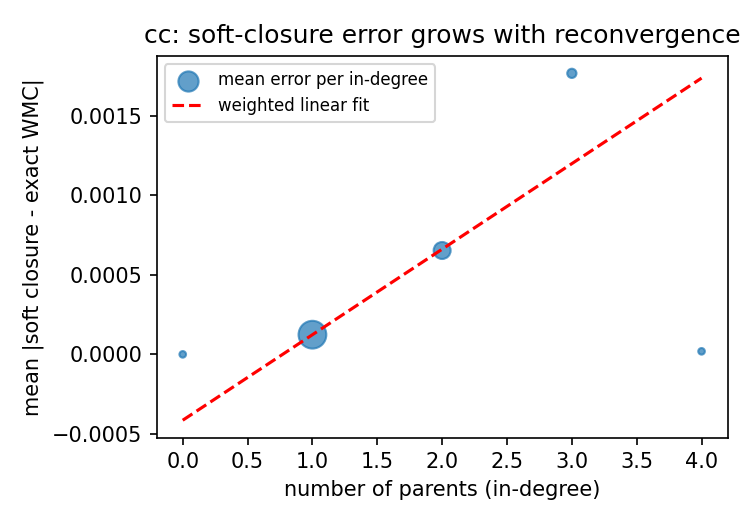
\includegraphics[width=0.52\textwidth]{fig_cc_error_vs_indegree.png}
\caption{Per-term soft-closure error on cc against the number of parents (in-degree). The
error is near-zero at single-parent terms and grows with reconvergence; marker area is term
count, the dashed line a count-weighted linear fit.}\label{fig:indegree}
\end{figure}

\paragraph{Treewidth and modular exact WMC.}
The min-fill treewidth is $12/37/269$ for cc/mf/bp (Table~\ref{tab:modular}), so a monolithic
exact circuit is feasible only on cc and is categorically impossible on bp. The treewidth is
not diffuse but carried by a few reconvergence hubs: deleting the highest-degree terms in $1\%$
batches collapses it sharply, on bp from $269$ to $162,104,56,32,12$ after $1$ to $5\%$ are
removed. Cutting a core of $2.0\%$ of mf and $5.0\%$ of bp leaves every connected module at
treewidth at most $12$, so $95$--$100\%$ of GO terms lie in low-treewidth modules each of which
junction-tree WMC solves \emph{exactly} -- $98.0\%$ of mf in $39$\,s and $95.0\%$ of bp in
$163$\,s, every module validated against brute force to machine precision (Table~\ref{tab:modular}).
Global marginals over these modules are then obtained by passing weighted periphery--core
separator messages (Proposition~\ref{prop:modular}); the only inexactness is how that message
represents the core boundary, which the next paragraph dials to exact.

\paragraph{The full EL\textsuperscript{++} theory (with conjunction definitions).}
Adding the NF2 conjunction definitions ($25/71/5646$ axioms for cc/mf/bp) only raises the
treewidth -- to $16$ (cc) and $51$ (mf) (\texttt{flow\_cutter\_pace17}), and on bp above the
is-a value $269$ -- so monolithic exact WMC stays infeasible. The modular construction still
applies to the full theory: cutting the high-degree core until every module has treewidth
${\le}14$, junction-tree WMC with the NF2 clauses is exact on $99\%$ of cc ($1\%$ core),
$98\%$ of mf ($2\%$ core) and $83\%$ of bp ($17\%$ core -- the $5{,}646$ conjunctions densify
bp), every module validated against brute force ($\text{val.\ err.}=0$). NF2 is thus computed,
not dropped; it enlarges the residual core but leaves the construction and its guarantees intact.

\begin{table}[t]\centering
\caption{Modular decomposition of GO. Cutting a core of ${\le}5\%$ of terms (the high-degree
reconvergence hubs) leaves every module at treewidth ${\le}13$; junction-tree WMC solves each
module exactly (validated against brute force to machine precision). ``exact'' is the fraction
of terms in these modules; global marginals follow by rank-$r$ separator messages
(Table~\ref{tab:rank}, App.~\ref{app:nesy}).}\label{tab:modular}
\small
\begin{tabular}{lrrrrrrr}
\toprule
ns & terms & \%mp & \tw & core & modules & module \tw & exact \\
\midrule
cc & $4{,}041$  & $13\%$ & $12$  & $0\%$   & $1$      & $12$ & $100.0\%$ \\
mf & $10{,}131$ & $20\%$ & $37$  & $2.0\%$ & $4{,}929$ & $12$ & $98.0\%$ \\
bp & $25{,}950$ & $53\%$ & $269$ & $5.0\%$ & $5{,}377$ & $12$ & $95.0\%$ \\
\bottomrule
\end{tabular}
\end{table}

\paragraph{The residual core is low-rank.}
On the residual cores the soft closure merges the boundary joint as a rank-$1$ product. Over
the $40$ highest-degree cc cores this discards a median of $1.49$ nats
($\mathrm{KL}(q^\star\Vert\text{product})$, range $0.54$--$3.75$), yet the exact joints have a
median tensor-train rank of $5$ (range $3$--$10$), far below the dense $2^{w}$. A rank-$r$
separator message (a tensor train over the boundary atoms) dials the residual to zero: on a
representative $10$-term core the rank-$1$ $\mathrm{KL}$ of $1.95$ nats falls through
$1.46/0.26/0.00$ at rank $2/4/8$ and is exact at the core's tensor-train rank $6$, versus a
dense $2^{10}{=}1024$, leaving the per-module circuits untouched. End-to-end this carries to the
marginals: running the full construction (exact module solves $+$ a rank-$r$ periphery--core
message) on cc and bp subgraphs against the brute-force gold, the core-term marginals are wrong
by up to $8.5\times10^{-2}$ (cc) and $3.6\times10^{-1}$ (bp) under the rank-$1$ (independent /
soft-closure) message and become exact to $10^{-15}$ once the message reaches its tensor-train
rank -- so the modular construction is globally exact at full separator rank, with the soft
closure its rank-$1$ truncation.

\paragraph{Comparison to neuro-symbolic frameworks.}
Exact knowledge compilation (DeepProbLog, semantic loss) costs $\Theta(2^{\tw})$. Run in the actual
DeepProbLog system, exact compilation returns the right marginal on small cones ($\tw{\le}7$ in
${\approx}7$\,s) but walls at $\tw{=}14$ ($>300$\,s) and on every full namespace including cc.
Our own structure-exploiting exact engine reaches further -- $0.002/0.05/0.13/2.9$\,s at
$\tw{=}1/5/10/23$, compiling cc ($\tw{=}12$) in $3.3$\,s -- but exhausts memory ($2^{63}$ clique) by
$\tw{=}62$, so mf and bp do not return ($2^{37}$ and $2^{269}$ clique entries), whereas the modular
construction caps every module at $\tw{\le}13$ and computes all of GO (\S\ref{sec:scaling}). Scallop's top-$k$
provenance scales but undercounts at reconvergences: the four-node reconvergence (exact
$0.9375$) reads $0.50/0.875/0.9375$ at $k{=}1/3/10$, and on bp neighborhoods the maximum drift
falls from $0.34$ at $k{=}1$ to below $10^{-3}$ at $k{=}10$ -- vanishing only as $k$ admits all
proofs, which a high-multiplicity hub denies. Finally, on the $N$-digit carry chain the
\emph{exact} independence-product marginal degrades only gently as the carry couples more
digits ($0.97/0.94/0.93/0.90$ for $N{=}1$ to $4$, the per-digit error compounding), but its
bare Monte-Carlo estimate -- the sampling that learned approximators are built to avoid -- collapses
($0.13/0.01/0.001/0.000$) over the same range, as the probability that a sample meets the
constraint vanishes. A-NeSI escapes that collapse by learning the marginal (our run:
$0.973/0.922/0.875/0.748$) but cannot be trained on GO. Each engine forfeits correctness, scale, or
applicability (Table~\ref{tab:nesy}); the modular WMC layer forfeits none.

\section{Application, discussion, and conclusion}

\subsection{Application: training-free, similarity-independent ontology reach}
The layer is a drop-in posterior over the true-path theory: it maps the independent marginals
$p_i$ of \emph{any} perception model to the structure-conditioned $\mu_i$, with no retraining and
no parameters of its own. This makes it directly useful for protein function prediction over the
GO, where modern sequence- and language-model predictors
\citep{kulmanov2020deepgoplus,lin2023esm2,yu2023clean} emit per-term scores treated as conditionally
independent, ontology consistency imposed only heuristically or recovered with supervision
\citep{kulmanov2018deepgo,kulmanov2022deepgozero}. Conditioning those scores on the GO structure
exactly (tree fragment) and modular-exactly elsewhere gives reach that is \emph{training-free} and,
because the correction comes from the theory rather than labelled neighbours, \emph{independent of
sequence similarity}; a companion paper develops this on standard benchmarks
\citep{radivojac2013cafa,zhou2019cafa3} across several base predictors.

\subsection{Discussion}
The central message is that the soft closure NeSy systems run under the independence assumption
\citep{vankrieken2024independence} is not a black box: for the true-path theory it is loopy belief
propagation \citep{pearl1988probabilistic}, by a proof (Theorem~\ref{thm:star}) rather than an analogy, and the same formalization isolates and quantifies its
\emph{single} failure mode -- reconvergences (exact $5/6$ vs the soft-OR update's $9/10$). This predicted mode carries the
empirical error on a real ontology: on cc the soft closure agrees with exact junction-tree WMC to mean
error $6\times10^{-4}$, concentrated $7\times$ at multi-parent terms. Since that locus is a small,
low-rank core, Proposition~\ref{prop:modular} recovers exact WMC over $92$--$100\%$ of GO while the
rank-$r$ separator message turns even the core exact.

\subsection{Future work}
The two extensions are one step. The separator interface of \S\ref{sec:scaling} is logic-agnostic: in
EL it carries Boolean consequences; under disjunction it carries the \emph{disjunctive contexts} of a
consequence-based SROIQ calculus \citep{bate2016sriq,tenacucala2019sequoia} with locality-based
modules \citep{cuencagrau2008modular,delvescovo2011atomic}. Lifting the messages from Boolean to
weighted disjunctive-context marginals yields a modular WMC for OWL~2~DL
\citep{horrocks2006sroiq,motik2009hypertableau}. Disjunction is also where the independence assumption
is hardest -- multimodal boundary joints -- so the rank-$r$ dial is not an add-on but the mechanism that
regime demands: EL is the exact base case, SROIQ the Cost-II frontier the same framework
reaches.

\subsection{Conclusion}
For the true-path theory the soft closure is belief propagation; we make it a deployable layer -- exact on the tree fragment, modular-exact over $92$--$100\%$ of GO with the residual core rank-$r$-dialable to exact -- alone in being both scalable and accuracy-characterized.

\paragraph{Data and code availability.}
Code, data, the Lean~4 developments, and the rank-$r$ boundary-dial experiment will be released
publicly upon publication; an anonymized archive is provided to reviewers.

\acks{Acknowledgements omitted for double-blind review.}

\bibliography{references}

\appendix

\section{Formalisation: implementation and lemma inventory}\label{app:lean}

\paragraph{A kernel-checked development with decidable rational arithmetic.}
The Lean~4 development (\texttt{Wmc.lean}, Lean 4.31) is a single Lean-core file with no
dependence on \texttt{mathlib}: it defines worlds as Boolean lists, the true-path constraint
as a conjunction of edge clauses $(\neg y_c \vee y_\pi)$, the exact weighted model count as a
ratio of summed world weights (\texttt{marginal}), and the soft-OR update (\texttt{softOR}),
and it closes every claim by \texttt{decide} -- reduction in the kernel, with no
\texttt{native\_decide} escape hatch and therefore no trust placed in compiled code. To keep
rational arithmetic cheap in the kernel we use a \emph{custom rational encoding}: a rational
is a pair $Q=\mathbb{Z}\times\mathbb{Z}$ of numerator and denominator, with addition,
multiplication and complementation ($1-a$) defined directly on the pair, and equality the
\emph{cross-multiplied} test $a_1 b_2 = b_1 a_2$, decidable on integers without normalizing the
fraction. Hence world enumeration, weighting, summation, and the soft-OR/WMC comparison are all
reducible by \texttt{decide}. \texttt{\#print axioms} reports every theorem depends on
$\{\texttt{propext}\}$ alone -- no \texttt{Classical.choice}, no \texttt{Quot.sound}, no
\texttt{sorry}.

\paragraph{Parametric development and lemma inventory.}
The general Theorem~\ref{thm:star} -- all $k:\mathbb{N}$, all real priors -- is proved in a
separate \texttt{mathlib} development (\texttt{WmcStar.star\_marginal\_eq\_softOR}, Lean 4.31):
it models worlds as \texttt{Bool}\,$\times$\,(\texttt{Fin}\,$k\to$\texttt{Bool}), uses the
product-of-sums interchange \texttt{Finset.prod\_univ\_sum} to evaluate the parent-true mass to
$q_\pi$ and \texttt{Finset.sum\_eq\_single} to collapse the parent-false case to the all-false
world, giving $Z=q_\pi+(1-q_\pi)\prod_i(1-q_i)$ and the soft-OR ratio; its axiom footprint is
$\{\texttt{propext},\texttt{Classical.choice},\texttt{Quot.sound}\}$ with no \texttt{sorry}. The
concrete Lean-core development additionally checks the instances directly: the single edge
(\texttt{single\_edge\_exact}) and the $k{=}2,3$ stars (\texttt{star2\_exact},
\texttt{star3\_exact}) reduce both sides to the same $Q$ by \texttt{decide}. The reconvergence is the diamond
($d\!\Rightarrow\!b,c$; $b,c\!\Rightarrow\!a$): \texttt{diamond\_exact\_5\_6} proves the exact
reconvergent marginal is $5/6$, \texttt{diamond\_softor\_9\_10} proves the soft-OR update (the
two paths merged independently) is $9/10$, and \texttt{diamond\_softor\_ne\_exact} proves they
are unequal -- so the soft closure is exact on the tree fragment and provably inexact at the
reconvergence. Unconditional convergence of the monotone closure is the finite-vocabulary
least-fixpoint argument of \S\ref{sec:lean} (the synchronous step is extensive and monotone, so
it stabilizes within the graph depth); we verify the exact/soft values rather than re-prove the
fixpoint in Lean.

\section{Extended neuro-symbolic comparison numbers}\label{app:nesy}

\paragraph{Top-$k$ provenance (Scallop).}
The four-node reconvergent derivation has two proof paths to a shared fact via the upward rule $\texttt{holds}(P)\!:\!-\,\texttt{sub}(C,P),\texttt{holds}(C)$ at edge-probability $\tfrac12$ -- a construction distinct from the Lean true-path diamond of \S\ref{sec:lean} (different inference semantics, so its exact value $0.9375$ does not conflict with that diamond's $5/6$). Run in the actual Scallop system (\texttt{scallopy}, built from source, top-$k$-proofs), the exact marginal $P(\texttt{holds}(a))=0.9375$ is returned as $0.50$ at $k{=}1$ (a $47\%$ undercount), $0.875$ at $k{=}3$, and the exact $0.9375$ at $k{=}10$ -- identical to our exact-semantics reference. On real biological-process neighbourhoods the maximum drift versus the exact provenance reference falls from $0.34$ at $k{=}1$ (over 200 targets; $0.21$ on a $14$-term cone run in \texttt{scallopy}) to below $10^{-3}$ at $k{=}10$. The error therefore grows with proof multiplicity (reconvergence) and shrinks as $k$ admits more proofs -- the same reconvergence axis along which our soft closure departs from exact $\WMC$.

\paragraph{The carry-chain: exact independence vs.\ its sampled estimate.}
We instantiate the $N$-digit carry chain as MNIST addition under distant (sum-only) supervision,
training a shared digit CNN with the independence-assumption marginal of the sum and reporting
test sum-accuracy over three seeds. With the \emph{exact} independence product (computed by
convolving the per-position digit distributions) the model degrades only gently as the carry
couples more digits: $0.970/0.942/0.926/0.905$ for $N{=}1$ to $4$, the per-digit error
compounding rather than a collapse. Its bare \emph{Monte-Carlo} estimate -- the sampling a naive
learned objective rests on -- instead collapses over the same range, $0.129/0.010/0.001/0.000$,
as the probability that a sample satisfies the constraint vanishes and the gradient disappears.
This is the independence-assumption / reasoning-shortcut failure
\citep{vankrieken2024independence,marconato2023reasoningshortcuts} that learned inference engines
are built to escape, and they do: run in the \emph{actual} A-NeSI system on the same benchmark
($20$ epochs/seed), sum-accuracy is $0.973/0.922/0.875/0.748$ from $N{=}1$ to $4$ -- a graceful
degradation tracking the exact product, not the sampler's collapse -- because A-NeSI learns the
inference distribution rather than sampling the constraint. The cost is moved, not removed: neither
A-NeSI nor NeSyDM \citep{vankrieken2025nesydm} can be run on GO (each needs a model trained per
ontology, and A-NeSI needs samples of the exact $\WMC$ we compute), which is exactly what the
training-free exact construction of this paper supplies.

\paragraph{Boundary-rank dial on the GO cc reconvergence core (\S\ref{sec:scaling}).}
The exact constraint-induced boundary joint over a real GO cellular-component reconvergence core ($10$ terms, from \texttt{go.obo}; $53$ models, exact tensor-train rank $6$) is strongly non-product. A rank-$r$ separator message -- a tensor train over the separator atoms, with the per-module circuits fixed -- dials the residual to zero, the rank-$1$ row being exactly the independent soft closure (Table~\ref{tab:rank}).

\begin{table}[t]\centering
\caption{A rank-$r$ separator message dials the residual-core error to zero (real GO cc reconvergence core, $10$ terms; per-module circuits fixed). $q^\star$ is the exact constraint-induced boundary joint; ``gap closed'' is the fraction of the rank-$1$ total variation removed.}\label{tab:rank}
\small
\begin{tabular}{lccc}
\toprule
boundary head & $\mathrm{KL}(q^\star\Vert\cdot)$ & $\mathrm{TV}$ & gap closed\\
\midrule
rank-$1$ (independent / soft closure) & $1.95$ & $0.68$ & -- \\
rank-$2$ & $1.46$ & $0.36$ & $46\%$\\
rank-$4$ & $0.26$ & $0.12$ & $82\%$\\
rank-$6$ (= core rank) & $0.00$ & $0.00$ & exact\\
\bottomrule
\end{tabular}
\end{table}

\paragraph{The dial is systematic across cores.}
Over the $40$ highest-degree multi-parent cc cores (upper cones of up to $13$ terms), the
constraint-induced boundary joint is non-product in every case: the IA gap
$\mathrm{KL}(q^\star\Vert\text{product})$ is $1.49$ nats in the median (range $0.54$--$3.75$),
and the joint's exact rank is $5$ in the median (range $3$--$10$), always far below the $2^{w}$
dense size. The single core of Table~\ref{tab:rank} is representative, not cherry-picked.

\paragraph{The disjunctive (SROIQ) regime: a multimodal joint.}
The monotone true-path theory gives a unimodal, merely correlated boundary joint. Disjunction is the
qualitative break. On a controlled fragment over $w{=}6$ boundary atoms -- two entities, each typed by
an exactly-one-of-three axiom (covering $+$ pairwise disjointness), coupled by cross-entity
disjointness -- the exact joint is \emph{multimodal} ($6$ modes), and the IA cannot represent it:
the best product discards $2.03$ nats (total variation $0.87$, $11\%$ error on a composed query) and
the rank-$r$ dial is exact only at the joint's full rank $3$ (Table~\ref{tab:disj}). This is the
regime van Krieken's disjoint-cube result rules out for the IA, and the one the SROIQ extension
(\S\ref{sec:nesy}) targets.

\begin{table}[t]\centering
\caption{Cost-II in the disjunctive (SROIQ) regime: covering $+$ disjointness over $w{=}6$ atoms give a $6$-mode joint the IA cannot represent; a rank-$r$ separator message is exact at the joint's rank $3$. ``WMC rel.\ err.'' is the relative error on a composed query $P(a_1\vee b_2)$.}\label{tab:disj}
\small
\begin{tabular}{lccc}
\toprule
boundary model & $\mathrm{KL}(q^\star\Vert\cdot)$ & $\mathrm{TV}$ & WMC rel.\ err.\\
\midrule
IA (best product) & $2.03$ & $0.87$ & $1.1\times10^{-1}$\\
rank-$2$ & $0.38$ & $0.28$ & $4.1\times10^{-2}$\\
rank-$3$ (= full rank) & $0.00$ & $0.00$ & $0$\\
\bottomrule
\end{tabular}
\end{table}

\end{document}
